\documentclass[10pt]{article}
\usepackage[utf8]{inputenc}
\usepackage[T1]{fontenc}
\usepackage{amsmath}
\usepackage{amsfonts}
\usepackage{amssymb}
\usepackage[version=4]{mhchem}
\usepackage{stmaryrd}
\usepackage{graphicx}
\usepackage[export]{adjustbox}
\graphicspath{ {./images/} }

\title{Ch/ChE 164 Winter 2024 }


\author{Homework Problem Set \#4}
\date{}


\begin{document}
\maketitle
Due Date: Thursday, February 15, 2024 @ 11:59pm PT

For all problems, please consider reasonable simplifications of your final results.

\begin{enumerate}
  \item (15 pts.) (Adapted from Callen). Consider a mixture of two non-identical monatomic ideal gases.
\end{enumerate}

\begin{itemize}
  \item Starting from the expression for the grand canonical partition function and taking the limit of small fugacity, show that the canonical partition function $Z$ is factorizable and
\end{itemize}


\begin{equation*}
Z=Z_{1} Z_{2}=\frac{1}{N_{1} !} q_{1}^{N_{1}} \frac{1}{N_{2} !} q_{2}^{N_{2}} \tag{1}
\end{equation*}


(You may wish to use the occupancy representation $\left.\mid n_{1} m_{1}, n_{2} m_{2} \ldots\right)$, where $n_{1}$ denotes occupancy of energy level 1 of gas 1 , and $m_{1}$ denotes occupancy of energy level 1 of gas 2 , etc.).

\begin{itemize}
  \item Compute the entropy and show that (comparing to the entropy of the two separate gases) there is an entropy of mixing of the form
\end{itemize}


\begin{equation*}
S_{\text {mixing }}=\left(-x_{1} \log x_{1}-x_{2} \log x_{2}\right) N k \tag{2}
\end{equation*}


where $N$ is the total number of particles.

\begin{enumerate}
  \setcounter{enumi}{1}
  \item In class we derived the heat capacity of the Fermi gas at low temperature by an intuitive argument, which $C_{v} \sim N k O\left(T / T_{F}\right)$. Here we will derive the precise form and constants (adapted from Callen).
\end{enumerate}

Denote the Fermi-Dirac distribution at temperature $T$ as $f(\epsilon, T)$ and the (temperature dependent) chemical potential by $\mu$ (note this is not the Fermi energy $\epsilon_{F}$ except when $T=0$ ). We will first derive a general result for an integral of the form (Sommerfeld expansion)


\begin{equation*}
I \equiv \int_{0}^{\infty} \phi(\epsilon) f(\epsilon, T) d \epsilon=\int_{0}^{\mu} \phi(\epsilon) d \epsilon+\frac{\pi^{2}}{6}(k T)^{2} \phi^{\prime}(\mu)+\frac{7 \pi^{4}}{360}(k T)^{4} \phi^{\prime \prime \prime}(\mu)+\ldots \tag{3}
\end{equation*}


a) (10 pts.) Integrate $I$ by parts, and let $\Phi \equiv \int_{0}^{\epsilon} \phi\left(\epsilon^{\prime}\right) d \epsilon^{\prime}$. Then expanding $\Phi(\epsilon)$ in a power series in $\epsilon-\mu$ to third order, deduce


\begin{equation*}
I=-\sum_{m=0}^{\infty} \frac{1}{m !} \frac{d^{m} \Phi(\mu)}{d \mu^{m}} I_{m} \tag{4}
\end{equation*}


where $I_{m}=\int_{0}^{\infty}(\epsilon-\mu)^{m} \frac{d f}{d \epsilon} d \epsilon=-\beta^{-m} \int_{-\beta \mu}^{\infty} \frac{e^{x}}{\left(e^{x}+1\right)^{2}} x^{m} d x$

b) (5 pts.) Show that only an exponentially small error is made by taking the lower limit of integration as $-\infty$, and that then all terms with $m$ odd vanish.

c) (5 pts.) Evaluate the first two non-vanishing terms and show that this agrees with the expansion of $I$.

d) (10 pts.) Using the result for $I$, express $N$ in the form of such an integral and obtain an expansion for $N(V, T, \mu)$ in terms of $k T / \mu$ (to second order). Verify that $T \rightarrow 0$ yields the relation between $N$ and $\epsilon_{F}$ derived in class.

e) (10 pts.) Invert this relationship to obtain $\mu(T)$ as a function of $k T / \epsilon_{F}$ (to second order) for fixed $N$.

f) (5 pts.) Similarly obtain an expansion for the internal energy $E$ as a function of $k T / \mu$ (to second order).

g) (5 pts.) Substituting in $\mu(T)$ into the energy expansion, obtain an expansion of $E$ in $k T / \epsilon_{F}$ to second order, and thus $C_{v}$. Hence see why we skipped the detailed computation in class.

\begin{enumerate}
  \setcounter{enumi}{2}
  \item (20 pts.) Show that for the Bose-Einstein and Fermi-Dirac gas at low density and/or high temperature the equation of state is given by
\end{enumerate}


\begin{equation*}
p=k T \rho\left(1 \mp \frac{\rho \Lambda^{3}}{2^{5 / 2}}+\ldots\right) \tag{5}
\end{equation*}


(1) $v_{1} T_{\mu_{2}} 2$ non-interacting gases

(i) $\begin{aligned} \text { gas 1: } n_{1}, n_{2}, n_{3} \ldots & N_{1} & =\sum_{i=1}^{\infty} n_{i} \\ \text { gas 2: } m_{1}, m_{2}, \cdots & N_{2} & =\sum_{i=1}^{\infty} m_{i}\end{aligned}$

$E_{v}=E_{v}^{\prime}+E_{v}^{2} \longleftarrow$ sum b/c non interacting otherwise need interaction potential term

$$
E^{\prime}=\sum_{i=1}^{\infty} n_{i} \epsilon_{i}^{(1)}+\sum_{i=1}^{\infty} m_{i} \epsilon_{i}^{(2)}
$$

\begin{itemize}
  \item grand canonical , $N, E$ can fluctuate
\end{itemize}

$$
\begin{aligned}
& \Xi=\sum_{v} e^{-\beta E_{v}+\beta \mu^{(1)} N_{1}+\beta \mu^{(2)} N_{2}} \\
& =\sum_{v} \exp \left(-\beta\left(\sum_{i=1}^{\infty} n_{i} \epsilon_{i}^{(1)}+\sum_{i=1}^{\infty} m_{i} t_{i}^{(2)}\right)+\beta \mu \sum_{i=1}^{(1)} n_{i}^{-}+\beta \mu^{(2)} \sum_{i=1}^{\infty} m_{i}\right) \\
& \Xi=\sum_{\operatorname{sn} 3} \sum_{\{m\}} \exp \left(-\beta\left[\sum_{i}^{\infty} n \epsilon_{i}^{(1)}+\sum_{i}^{\infty} m_{i} \epsilon^{(2)}-\sum_{i}^{\infty} \mu_{i}^{(1)} n_{i}-\sum_{i}^{\infty} \mu_{i}^{(2)} m\right]\right)
\end{aligned}
$$

\begin{itemize}
  \item move sums from exp to product
\end{itemize}

$$
\begin{aligned}
& \Xi=\prod_{i} \sum_{n_{i}} \sum_{m_{i}} \exp \left(-\beta\left[n_{i} t_{i}^{(1)}+m_{i} t_{i}^{(2)}-\mu_{i}^{(1)} n_{i}-\mu_{i}^{(2)} m_{i}\right]\right) \\
& =\underbrace{}_{i} \sum_{n_{i}} \exp \left(\beta n_{i}\left(\mu_{i}^{(1)}-\epsilon_{i}^{(1)}\right)\right) \pi_{i} \sum_{m_{i}} \frac{\exp \left(\beta m_{i}\left[\mu_{i}^{(2)}-\epsilon_{i}^{(2)}\right]\right)}{\Xi_{2}} \\
& \Xi=\Xi_{1} \Xi_{2}
\end{aligned}
$$

each obey
$F D, B E$ stats: $B E: n_{i}, m_{i}$ can be any any

FD: ni, mi can be o, 1 only

$$
=\prod_{i} e^{\left(\beta \mu_{i}-\epsilon_{i}\right)^{n_{i}}} \prod_{i} e^{\left(\beta \mu_{i}-\epsilon_{i}\right)^{m}}
$$

$B E: \Xi=\prod_{i}\left(1-e^{\beta \mu-\beta t_{i}}\right)^{-1}, F D: \Pi_{i}\left(1+e^{\beta \mu-\beta t_{i}}\right)$

$$
\begin{aligned}
\Xi & =\prod_{i}\left(1 \mp e^{\beta \mu-\beta \epsilon_{i}}\right) \mp 1 \\
\ln \Xi & =\mp \ln \prod_{i}\left[1 \mp e^{\beta \mu-\epsilon_{i}}\right]=\mp \sum_{i} \ln \left[1 \mp e^{\beta \mu-c_{i}}\right]
\end{aligned}
$$

Chow fugacity $e^{\beta \mu} \ll 1, T . E$.

$\ln (1+x)$ for small $x: \longrightarrow x-\frac{x^{2}}{2}+\frac{x^{3}}{3}+\cdots$

$$
\ln \sqsubseteq=\mp \sum_{i}\left(\mp e^{\beta \mu-t_{i}}\right)=+e^{\beta \mu} \sum_{i} e^{\epsilon_{i}}=e^{\beta \mu} q
$$

$q$ is single particle partition $\mathrm{f} \times \mathrm{n}$

$$
\begin{aligned}
& \Xi=\exp \left(e^{\beta \mu} q\right), e^{x}=\sum_{N=0}^{\infty} \frac{1}{N !} x^{N} \\
& \Xi=\sum_{N=0}^{\infty} \frac{1}{N !} q^{N} e^{\beta \mu N}=\Xi_{1} \Xi_{2} \\
& \Xi=\sum_{N=0}^{\infty} \frac{1}{N !} q^{N} e^{\beta M^{(1)} N} \sum_{M}^{\infty} \frac{1}{M !} q^{M} e^{\beta M^{(2)} M}=\sum_{N}^{\infty} z e^{\beta \mu N} \\
& \rightarrow Z=\left(\frac{1}{N} ! q^{N}\right)\left(\frac{1}{M !} q^{M}\right) \\
& Z=Z_{1} Z_{2}=\frac{1}{N_{1} !} q_{1}^{N} \frac{1}{N_{2}} q_{2}^{N_{2}}
\end{aligned}
$$

(ii) find entropy (thermos approach)

Smixing $=S_{\text {mix }}-S_{1} \cdot S_{2}$

$$
\begin{aligned}
& F=-k T \ln z \\
& S=-\left(\frac{\delta F}{\delta T}\right)_{N_{1}, N_{2}, v}, q=\frac{v}{\Lambda^{3}}=\left(\frac{2 m k T}{n^{2}}\right)^{3 / 2} v \\
& \left.S_{1}=-k N_{1} \ln \rho_{1}^{*} \Lambda^{3}+\frac{5}{2} k N_{1}\right\} \rho_{1}^{*}, \rho_{2}^{*} b / c \\
& \text { occupy } v_{1}, v_{2} \neq v \\
& \rho_{2}=-k N_{2} \ln \rho_{2}^{*} \Lambda^{3}+\frac{5}{2} k N_{2}=\frac{N}{V_{1}}, \frac{V_{1}}{v}=x_{1} \\
& F_{\operatorname{mix}}=-k T \ln \left(z_{1} 2_{2}\right)=-k T \ln \left(\frac{1}{N_{1} !} q_{1}^{N_{1}} \frac{1}{N_{2}} ! q_{2}^{N_{2}}\right) \\
& =-k T\left[N_{1} \ln N_{1}-N_{1}+N_{1} \ln q_{1}+N_{2} \ln N_{2}-N_{2}+N_{2} \ln q_{2}\right]
\end{aligned}
$$

$$
\begin{aligned}
& S_{\text {mix }}=-\left(\frac{\delta F_{\text {mix }}}{\delta T}\right)_{N_{1} N_{2}, v}=-k \ln \frac{1}{N_{1} !} \frac{1}{N_{2} !}-\frac{\delta}{\delta T} k T \ln q_{1}^{N_{1}} q_{2}^{N_{2}} \\
& =-k \ln \frac{1}{N_{1} !} \frac{1}{N_{2} !}-\frac{\delta}{\delta T} k T\left(N_{1} \ln \left(\frac{2 m k}{n^{2}}\right)^{3 / 2} V+N_{2} \ln \left(\frac{2 m k}{\hbar^{2}}\right)^{3 / 2} V\right. \\
& \left.+\frac{3}{2}\left(N_{1}+N_{2}\right) \ln T\right) \\
& =-k\left[\ln \frac{1}{N_{1}} ! \frac{1}{N_{2}} !+\ln \left(\frac{2 m k}{\hbar}\right)^{3 / 2} V\left(N_{1}+N_{2}\right)\right]-k \ln T\left(N_{1}+N_{2}\right) \\
& +\frac{2}{2} \frac{1}{T}\left(N_{1}+N_{2}\right) k T \\
& =k\left(N_{1}+N_{2}-N_{1} \ln \left(\frac{2 m k}{\hbar^{2}}\right)^{3 / 2} \rho_{1}-N_{2} \ln \left(\frac{2 m k}{\hbar^{2}}\right)^{3 / 2} \rho_{2}\right. \\
& \left.-\frac{3}{2}\left(N_{1}+N_{2}\right)(\ln T-1)\right)=k\left(-N_{1} \ln \rho_{1} \Lambda^{3}-N_{2} \ln \rho_{2} \Lambda^{3}+\frac{5}{2}\left(N_{1}+N_{2}\right)\right] \\
& S_{\text {mixing }}=S_{\text {mix }}-S_{1}-S_{2}=\frac{S}{2} k N_{1}+\frac{S}{2} k N_{2}-N_{1} k \ln \rho_{1} \wedge^{3} \\
& -N_{2} \ln \rho_{2} \Lambda^{3}-\frac{5}{2} K N_{1}+K N_{1} \ln \rho_{1}^{*} \Lambda^{3} \\
& +k N_{2} \ln _{2}^{*} \cap^{3} \\
& \text { mixing }=N k\left(-x_{1} \ln \rho_{1}-x_{1} \pi \pi \wedge^{3}-x_{2} \ln \rho_{2}\right. \\
& -x_{2} \operatorname{tn} \Lambda^{3}+x_{1} \ln \rho_{1}^{*}-x_{1} \operatorname{tn} \Lambda^{3} \\
& \left.+x_{2} \ln \rho_{2}^{*}-x_{2}+n \Lambda^{3}\right)
\end{aligned}
$$

\begin{itemize}
  \item no variation in $\Lambda$, but variation in $\rho(v)$
\end{itemize}

$$
\begin{array}{r}
\text { Smixing }=N_{k}\left(-x_{1} \ln \left(\frac{N_{1}}{V} \cdot \frac{V_{1}}{N_{1}}\right)-x_{2} \ln \left(\frac{N_{2}}{V} \cdot \frac{V_{2}}{N_{2}}\right)\right) \\
\frac{V_{1}}{V}=\frac{N_{1}}{N_{1}+N_{2}}=x_{1}, \frac{V_{2}}{V}=\frac{N_{2}}{N_{1}+N_{2}}=x_{2} \\
\text { Smixing }=N_{k}\left(-x_{1} \ln x_{1}-x_{2} \ln x_{2}\right)
\end{array}
$$

(2) Cr of Fermions

$$
f(t, T)=\left(e^{\beta(t-\mu)}+1\right)^{-1}, I \equiv \int_{0}^{\infty} \phi(t) f(t, T) d t
$$

(a) integrate by parts gives arg of $\phi$

$$
\begin{aligned}
& u=f(t, T), d u=\frac{\delta f}{\delta t} d t \\
& d v=\phi(t) \quad v=\int \phi(\epsilon) d t \\
& I=u v-\int v d u=\left.f(t, T) \int_{0}^{t} \phi\left(t^{\prime}\right) d t^{\prime}\right|_{0} ^{\infty} \quad f(\infty)=0 \\
& \quad-\int_{0}^{0} \frac{\delta f}{\delta t}\left[\int_{0}^{t} \phi\left(t^{\prime}\right) d t^{\prime}\right] d t \\
& I \pm-\int_{0}^{\infty} \frac{\delta f}{\delta t} \Phi(t) d t
\end{aligned}
$$

\begin{itemize}
  \item Taylor Expand around $\mu$
\end{itemize}

$$
\begin{gathered}
\Phi(\mu)=\sum_{m=0}^{\infty} \frac{1}{m !}\left(\frac{\delta^{m} \Phi}{\delta \epsilon^{m}}\right)(t-\mu)^{m} \\
I=-\sum_{m=0}^{\infty} \frac{1}{m !}\left(\frac{\delta^{m} \Phi}{\delta \epsilon^{m}}\right) \int_{0}^{\infty} \frac{\delta f}{\delta t}(t-\mu)^{m} d t \\
I=-\sum_{m=0}^{\infty} \frac{1}{m !}\left(\frac{\delta^{m} \Phi(\mu)}{\delta \epsilon^{m}}\right) I_{m}
\end{gathered}
$$

(b)

$$
\begin{aligned}
& \text { (b) } I_{m}=\int_{-\beta \mu}^{\infty} \frac{e^{x} x^{m}}{\left(e^{x}+1\right)^{2}} d x \text {, argue } \int_{-\beta \mu} \rightarrow \int_{-\infty} \\
& I_{m}=\int_{0}^{\infty} \frac{\delta f}{\delta t}(\epsilon-\mu)^{m} d t=\int_{0}^{\infty} \frac{\beta e^{\beta(t-\mu)}}{\left(e^{\beta(t-\mu)+1)^{2}}\right.}(t-\mu)^{m} d t \\
& x=t-\mu \quad=-\beta^{-m} \int_{-\beta \mu}^{\infty} \frac{e^{x}}{\left(e^{x}+1\right)^{2}} x^{m} d x
\end{aligned}
$$

need to show $\int_{-\infty}^{-\beta \mu} \frac{e^{x} x^{m}}{\left(e^{x}+1\right)^{2}} d x$ is exponentially $\sim \int_{-\infty}^{-\beta \mu} e^{x} x^{m} \leq \int_{-\infty}^{-\beta \mu} \frac{e^{x} x^{m}}{\left(e^{x}+1\right)^{2}} d x \quad b / c$ smallest value of $\leadsto \int_{-\infty}^{-\beta \mu} e^{x} x^{m}, e^{x}$ donimates $x^{m} \$ e^{x}$ is exponentially small for all $x<0$ and $\beta \mu>>1$

$$
\begin{aligned}
& I_{m}=-\beta^{-m} \int_{-\infty}^{\infty} \frac{e^{x} x^{m}}{\left(e^{x}+1\right)^{2}} d x+\beta^{m} \int_{-\infty}^{-\beta \mu} \frac{e^{x} x^{m}}{\left(e^{x}+1\right)^{2}} d x \\
& I_{m} \simeq-\beta^{-m} \int_{-\infty}^{\infty} \frac{e^{x} x^{m}}{\left(e^{x}+1\right)^{2}} d x
\end{aligned}
$$

\begin{itemize}
  \item when $m$ is odd $\rightarrow x^{m}$ is oddfxn $\left(x, x^{3}, x^{s}\right.$ even $f_{x n}: \int_{-\infty}^{0} \cdots=\int_{0}^{\infty}$ v. $\left.x^{2}, x^{4}\right)$
\end{itemize}

odd $f \times n: \quad \int_{-\infty}^{0}=-\int_{0}^{\infty} \rightarrow \int_{-\infty}^{\infty}=0$

because we are taking $\int_{-\infty}^{\infty}, x^{m}$ where $m$ is odd cancel ( $e^{x} /\left(e^{x}+1\right)^{2}$ is even)

(C) (5 pts.) Evaluate the first two non-vanishing terms and show that this agrees with the
expansion of $I$.

$$
\begin{aligned}
& I_{0}=(1) \Phi(\mu) \int_{-\infty}^{\infty} \frac{e^{x}}{\left(e^{x}+1\right)^{2}} d x=\Phi(\mu)\left[\left(e^{x}-1\right)\right]_{-\infty}^{1} \\
& I_{0}=\underline{P}(\mu)=\int_{0}^{t} \phi\left(t^{\prime}\right) d t^{\prime} \\
& I_{2}=+\frac{1}{2 !}\left(\frac{\delta^{2} \Phi(\mu)}{\delta t^{2}}\right) \int_{-\infty}^{\infty} \frac{x^{2} \cdot e^{x}}{\left(e^{x}+1\right)^{2}} d x \\
& \Phi \equiv \int_{0}^{\epsilon} \phi\left(\epsilon^{\prime}\right) d \epsilon^{\prime}
\end{aligned}
$$

\begin{center}
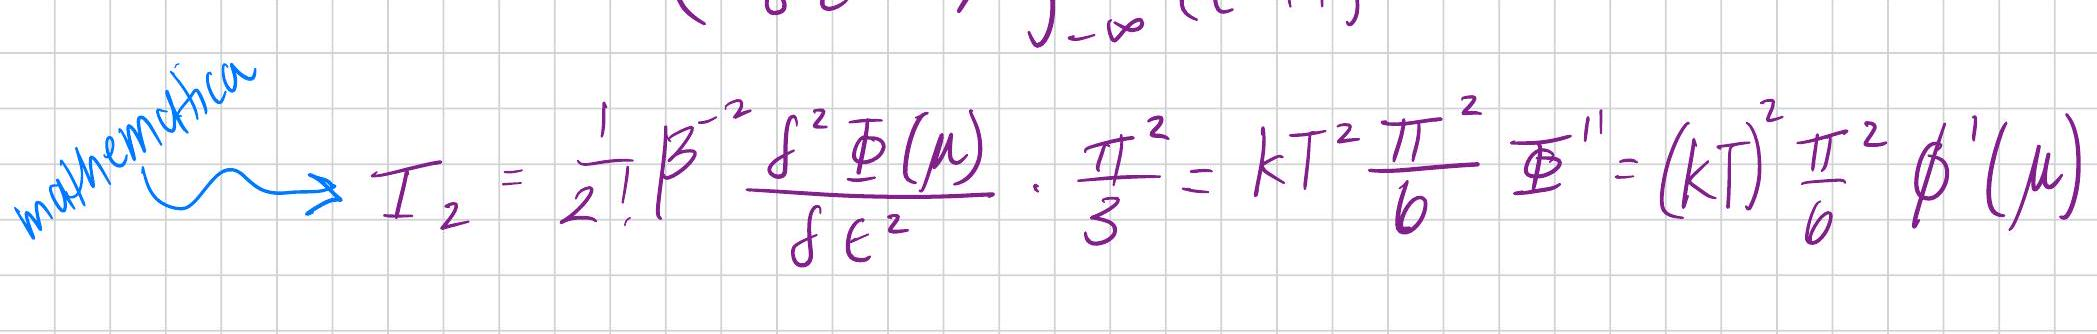
\includegraphics[max width=\textwidth]{2024_02_15_8bd07fd17573a85b0312g-09}
\end{center}

$$
\begin{aligned}
& I \equiv \int_{0}^{\infty} \phi(\epsilon) f(\epsilon, T) d \epsilon=\underbrace{\int_{0}^{\mu} \phi(\epsilon) d \epsilon}_{\checkmark}+\underbrace{\frac{\pi^{2}}{6}(k T)^{2} \phi^{\prime}(\mu)}_{\checkmark}+\frac{7 \pi^{4}}{360}(k T)^{4} \phi^{\prime \prime \prime}(\mu)+\ldots
\end{aligned}
$$

(d)

d) (10 pts.) Using the result for $I$, express $N$ in the form of such an integral and obtain an expansion for $N(V, T, \mu)$ in terms of $k T / \mu$ (to second order). Verify that $T \rightarrow 0$ yields the relation between $N$ and $\epsilon_{F}$ derived in class.

$$
N=\sum_{\alpha}\left\langle n_{\alpha}\right\rangle=\int_{0}^{\infty} \phi(\varepsilon) f(t, T) d t
$$

$L$ density of states for particle \#

(a) 89

eq

$$
\begin{aligned}
& \phi(t) \rightarrow \rho(t)=\frac{V}{2 \pi^{2}} \cdot \frac{(2 m)^{3 / 2}}{\hbar^{3}} t^{1 / 2} \\
& \phi^{\prime}(t) \rightarrow \rho^{\prime}(\mu)=\frac{V}{4 \pi^{2}} \frac{(2 m)^{3 / 2}}{\hbar^{3}} \mu^{-1 / 2} \\
& N=\int_{0}^{\mu} \rho(t) d t+\frac{\pi^{2}}{6}(k T)^{2} \frac{V}{4 \pi^{2}}\left[\frac{(2 m)^{3 / 2}}{\hbar^{3}} t^{-1 / 2}\right]+\ldots \\
& N=\frac{2}{3} \cdot \frac{V}{2 \pi^{2}} \frac{(2 m)^{3 / 2}}{\hbar^{3}} \mu^{3 / 2}+\frac{\pi^{2}}{6}(k T)^{2} \frac{V}{4 \pi^{2}}\left[\frac{(2 m)^{3 / 2}}{\hbar^{3}} \mu^{-1 / 2}\right]+\cdots \\
& N\left(V_{1} T, \mu\right)=\frac{V}{3 \pi^{2}}\left(\frac{2 m}{\hbar^{2}}\right)^{3 / 2} \mu^{3 / 2}\left[1+\frac{\pi^{2}}{8}\left(\frac{k T}{\mu}\right)^{2}\right] \\
& k T \rightarrow 0, \quad \mu=\epsilon_{F} \\
& {\left[N\left(V, T, \epsilon_{F}\right)=\frac{V}{3 \pi^{2}}\left(\frac{2 m}{\hbar^{2}}\right)^{3 / 2} \epsilon_{F}^{3 / 2}\right]}
\end{aligned}
$$

(e) 10 pts.) Invert this relationship to obtain $\mu(T)$ as a function of $k T / \epsilon_{F}$ (to second order) for fixed $N$.

$$
\begin{gathered}
N(V, T, \mu)=N\left(V, T, \epsilon_{F}\right) \\
\frac{v}{\beta \pi^{2}}\left(\frac{2 m}{\pi^{2}}\right)^{3 / 2} \mu^{3 / 2}\left[1+\frac{\pi^{2}}{8}\left(\frac{k T}{\mu}\right)^{2}\right]=\frac{V}{\beta \pi^{2}}\left(\frac{2 m}{\hbar^{2}}\right)^{3 / 2} \epsilon_{F}^{3 / 2} \\
\left(\frac{\mu}{\epsilon_{F}}\right)^{3 / 2}\left[1+\frac{\pi^{2}}{8}\left(\frac{k T}{\mu}\right)^{2}\right]=1 \\
\left(\frac{\mu}{\epsilon_{F}}\right)^{3 / 2}=1-\frac{\pi^{2}}{8}\left(\frac{k T}{\epsilon_{F}}\right)^{2}\left(\frac{\mu}{\epsilon_{F}}\right)^{-1 / 2} \text { low } T \\
\frac{\mu}{\epsilon_{F}} \approx\left(1-\frac{\pi^{2}}{8}\left(\frac{k T}{\epsilon_{F}}\right)^{2}\right)^{2 / 3} \\
\mu \approx t_{F}\left[1-\frac{\pi^{2}}{12}\left(\frac{k T}{\epsilon_{F}}\right)^{2}\right]
\end{gathered}
$$

(f)

( 5 pts.) Similarly obtain an expansion for the internal energy $E$ as a function of $k T / \mu$ (to second order).

$$
E=\int_{0}^{\infty} \phi(\varepsilon) f(t, T) d t
$$

density of states for energy

$$
\begin{aligned}
& \phi(t) \rightarrow \int \in(t)=\left.\int \frac{V}{2 \pi^{2}} \cdot \frac{(2 m)^{3 / 2}}{\hbar^{3}} t^{3 / 2} \rightarrow \frac{2}{S} \cdot \frac{V}{2 \pi^{2}}\left(\frac{2 m}{\hbar^{2}}\right)^{3 / 2} \epsilon^{5 / 2}\right|_{0} ^{\mu} \\
& \phi^{\prime}(t) \rightarrow \epsilon \rho^{\prime}(t)=\frac{V}{2 \pi^{2}} \frac{(2 m)^{3 / 2}}{\hbar^{3}} \cdot \frac{3}{2} \epsilon^{\prime / 2} \quad \text { change to } \mu \\
& E=\frac{V}{S \pi^{2}}\left(\frac{2 m}{\hbar^{2}}\right)^{3 / 2} \mu^{5 / 2}+\frac{\pi^{2}}{6}(k T)^{2}-\frac{2}{5} \cdot \frac{V}{2 \pi^{2}}\left(\frac{2 m}{\hbar^{2}}\right)^{3 / 2} \mu^{1 / 2}
\end{aligned}
$$

$$
E=\frac{V}{S \pi^{2}}\left(\frac{2 m}{\hbar^{2}}\right)^{3 / 2} \mu^{s / 2}\left[1+\frac{\pi^{2}}{6}\left(\frac{k T}{\mu}\right)^{2}\right]
$$

(9)

g) (5 pts.) Substituting in $\mu(T)$ into the energy expansion, obtain an expansion of $E$ in $k T / \epsilon_{F}$ to second order, and thus $C_{v}$. Hence see why we skipped the detailed computation in class.

$$
\begin{aligned}
& (v, T, \mu)=\frac{v}{3 \pi^{2}}\left(\frac{2 m}{\pi^{2}}\right)^{3 / 2} \mu^{3 / 2}\left[1+\frac{\pi^{2}}{8}\left(\frac{k T}{\mu}\right)^{2}\right] \\
& E=\frac{3}{5} N \epsilon_{F}\left[\left(\frac{\mu}{t_{F}}\right)^{5 / 2}+\frac{5 \pi^{2}}{24}\left(\frac{k T}{\epsilon_{F}}\right)^{2}\left(\frac{\mu}{\epsilon_{F}}\right)^{1 / 2}\right] \\
& E=\frac{3}{5} N t_{F}\left[\left(1-\frac{\pi^{2}}{12}\left(\frac{k F}{\epsilon_{F}}\right)^{2}\right]^{5 / 2}+\frac{\pi^{2}}{24}\left(\frac{k T}{\epsilon_{F}}\right)^{2}\left[1-\frac{\pi^{2}}{12}\left(\frac{k T}{\epsilon_{F}}\right)^{2}\right]^{1 / 2}\right] \\
& \longrightarrow C_{V}=\frac{\delta E}{\delta T}=2\left(\frac{3}{2} t_{F}+\frac{\pi^{2}}{4} N \epsilon_{F}\left(\frac{k T}{\epsilon_{F}}\right)^{2} N t_{F}\left(\frac{k}{\epsilon_{F}}\right)^{2} T\right.
\end{aligned}
$$

$$
C_{V}=\frac{\pi^{2}}{2} N \frac{k^{2}}{t_{F}} T
$$

I used these,

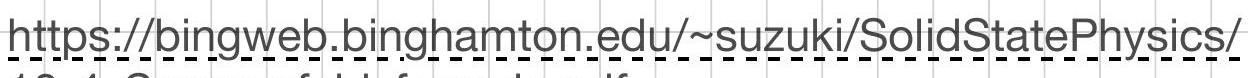
\includegraphics[max width=\textwidth, center]{2024_02_15_8bd07fd17573a85b0312g-12(1)}
10-4 Sommerfeld formula.:pdf

\begin{center}
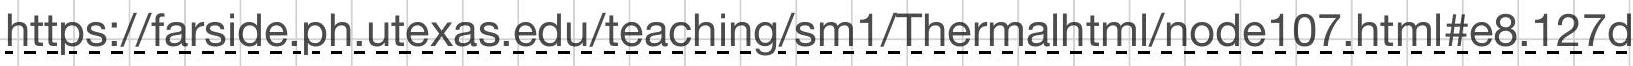
\includegraphics[max width=\textwidth]{2024_02_15_8bd07fd17573a85b0312g-12}
\end{center}

(3) (20 pts.) Show that for the Bose-Einstein and Fermi-Dirac gas at low density and/or high fem

$$
p=k T p\left(1+\frac{\alpha^{3} z^{3}}{+z^{3}}+\ldots\right) .
$$

$\longrightarrow$ online lecture 8 notes

alow density limit $e^{\beta \mu} \ll 1, e^{\beta \mu}=z^{\prime \prime}$ 'fugacity'

\begin{itemize}
  \item FD -BE partition fan
\end{itemize}

$$
\begin{aligned}
\ln \Xi & =\sum_{i} \ln \left(1 \mp e^{\beta \mu-\beta \varepsilon_{i}}\right)^{\mp 1} \\
& =\frac{1}{8} \cdot \frac{V}{4 \pi^{3} \hbar^{3}} \int_{0}^{\infty} d p 4 \pi p^{2} \ln \left(1 \mp e^{\beta \mu-\beta p^{2} / 2 m}\right)^{\mp 1} \\
& =\frac{V}{1^{3}} \frac{4}{\sqrt{\pi}} \int_{0}^{\infty} d x \cdot x^{2} \ln \left(1 \mp\left\{e^{-x^{2}}\right)^{\mp 1}\right.
\end{aligned}
$$

$\{\rightarrow 0$, expand series in $\xi$ and integrate

$$
\begin{gathered}
=\frac{V}{\Lambda^{3}}\left(\frac{4}{\sqrt{\pi}}\right)\left(\frac{\sqrt{\pi}}{4}\right)\left[\sum_{n=1}^{\infty}(F \mid)^{n+1} \frac{\xi^{n}}{n^{s / 2}}\right]=\frac{V}{\Lambda^{3}} f_{s / 2}(\xi) \\
d W=-S d T-P d V-N d \mu \\
W=-k T \ln \bar{U} \\
P=-\left(\frac{\delta W}{\delta V}\right)_{T, \mu}=k T\left(\frac{1}{\Lambda^{3}} f_{s / 2}(\xi)\right)
\end{gathered}
$$

$$
\begin{aligned}
& N=-\left(\frac{\delta W}{\delta \beta \mu}\right)_{T, V}=\left(\frac{k T \delta \ln \Xi}{\delta \mu}\right)=\xi k T\left(\frac{V}{\Lambda^{3}} f_{s / 2}(\xi)\right) \\
& \beta P(T, \mu)=\frac{f_{s / 2}(\xi)}{\Lambda^{3}}, \beta N=\frac{V}{\Lambda^{3}} f_{3 / 2}(\xi)
\end{aligned}
$$

expand in

$$
\begin{aligned}
& { }^{n} f_{s / 2}(\xi)=\left\{F \frac{\xi^{2}}{2^{s / 2}} \cdots\right. \\
& \beta P=\frac{1}{1^{3}}\left(\xi^{1}+\frac{\xi^{2}}{2^{5 / 2}} \cdots\right) \\
& \frac{N}{V}=\rho=\frac{1}{1^{3}}\left(\xi+\xi^{2} / 2^{3 / 2} \cdots\right)
\end{aligned}
$$

$\beta P=\rho$ ideal gas

need to get $\beta P=\rho f(\xi)=\rho\left(\Lambda^{3} \rho\right)$ viral expansion $\rightarrow$ eliminate $\{$ from $\rho$

plug $\{$ in

$$
\Lambda^{3} \rho=\left\{\mp \frac { \gamma ^ { 2 } } { 2 ^ { 3 / 2 } } \rightarrow \left\{=\Lambda^{3} \rho \mp \frac{\xi^{2}}{2^{3 / 2}}\right.\right.
$$

to $\beta P$

$$
\begin{aligned}
& \xi=\Lambda^{3} p \mp \frac{\left(\Lambda^{3} p\right)^{2}}{2^{3 / 2}} \\
& P=k T \frac{1}{\Lambda_{3}}\left(\Lambda^{3} p \mp \frac{\left(\Lambda^{3} p\right)^{2}}{2^{2 / 3}} \mp\right. \\
& P=k T p\left(1 \mp \frac{\Lambda^{3} p}{\left.2^{2 / 5} \cdots\right)}\right.
\end{aligned}
$$

$$
P=k T \frac{1}{\Lambda_{3}}\left(\Lambda^{3} p \mp \frac{\left(\Lambda^{3} p\right)^{2}}{2^{2 / 3}} \mp \frac{\left(\Lambda^{3} p\right)^{2}}{2^{5 / 2}} \cdots\right)
$$


\end{document}